
\section{Ejercicio 1}
\subsection{Introducción}
El problema consiste en hallar el camino que utilice la mayor cantidad posible de portales para llegar desde el piso 0 al N.
En este contexto, los portales solo llevan a pisos superiores, nunca bajan.
Se garantiza que existe un camino m\'aximo entre los pisos mencionados y que no hay m\'as de un portal que comunique el mismo par de pisos.

\subsection{Desarrollo}
A fin de encontrar el camino mas largo en tiempo cuadrático sobre la cantidad de pisos, planteamos una solución con programación dinámica.
Podemos definir recursivamente el largo del camino con la máxima cantidad de portales atravesados para llegar a un piso dado hasta el piso n como:

\begin{center}
$P_N(p) =max_{p' \in suc(p)}\{ 1 + P_N(p')\}$
\end{center}

Donde $suc(p)$ son los pisos que tienen un portal con origen en $p$.

Implementamos este comportamiento con una representación como listas de antecesores.

Partimos desde el último piso, indicándolo como accesible, e iteramos hacia abajo. 
Para cada piso, si es accesible desde el piso N, por cada antecesor calculamos el máximo entre el valor ya calculado (si lo hay) 
y la cantidad de portales hasta el enésimo piso sumado uno, y memorizamos este resultado. Podría existir un valor previo si el antecesor en cuestión también lo es para algún piso superior.
Hecho esto, marcamos sus antecesores como accesibles y continuamos iterando hasta llegar al piso 0.

Cuando esto suceda, como sabemos que existe camino entre último piso y la planta baja, habremos calculado $P_N(0)$.

Implementamos este comportamiento con el siguiente algoritmo:

\begin{algorithm}
\caption{Camino Máximo}\label{alg-ej1}
\begin{algorithmic}[1]
\Procedure{CaminoMáximo}{}
\State $\textit{pisos} \gets \text{lista de antecesores}$
\State $\textit{accesible} \gets \text{arreglo de tamaño }N$
\State $\textit{maximoDesdeN} \gets \text{arreglo de tamaño }N$
\State Inicializar $accesible$ en 0 para todas sus posiciones
\State Inicializar $maximoDesdeN$ en 0 para todas sus posiciones
\State $accesible_N \gets true $ 

\for {$p = N\text{ hasta }0$}
\State $piso \gets pisos_i$
\If {$\textit{accesible}_p$}
\for{$antecesor$ en $piso.antecesores$}
\State $maximo \gets\max\{maximoDesdeN_{piso.numero} + 1 , maximoDesdeN_{antecesor}\}$
\State $maximoDesdeN_{antecesor} \gets maximo$
\State $accesible_{antecesor} \gets true$
\EndFor
\EndIf
\EndFor  
\Return $maximoDesdeN_{0}$
\EndProcedure
\end{algorithmic}
\end{algorithm}

En el código utilizamos una estructura propia para representar cada piso, que agrupa el número de piso y una lista de los números de los antecesores. Ésta lista se implementa como una lista enlazada, por lo que tiene costo de inserción constante. En el algoritmo descrito, $pisos$ es una arreglo de estas estructuras, ordenada por numero de piso cuando es construida. Esto tiene lugar de la siguiente manera: 

\begin{algorithm}
\caption{Inicialización Camino Máximo}\label{init-ej1}
\begin{algorithmic}[2]
\Procedure{Init}{}
\State $\textit{pisos} \gets \text{arreglo de tamaño }N$

\for {$i = 0\text{ hasta }N$}
\State $antecesores \gets \text{nueva Lista de }int$
\State $piso \gets \text{nuevo }\textit{Piso(i,antecesores) }$
\State $pisos_i \gets piso $
\EndFor  

\for{$portal$ en $portales$}
\State $pisos_{portal.hasta}.antecesores.agregarAtras( portal.desde )$
\EndFor

\EndProcedure
\end{algorithmic}
\end{algorithm}



\subsection{Correctitud}

Como iteramos desde el piso N al 0, partiendo de $P_N(N) = 0$, cuando estemos iterando sobre el piso $p$, si hay portales que lo conecten con el último piso, ya tendremos $P_N(p)$ correctamente calculado y memorizado.
Podemos afirmar esto porque como los portales solo suben, el piso $p$ no puede ser antecesor de ningún piso sobre el cual nos falte iterar, pues como puede verse en el algoritmo \ref{alg-ej1}, $maximoDesdeN$ (el vector donde memorizamos los resultados de $P_N$) solo se modifica en las posiciones correspondientes a antecesores del piso sobre el cual se itera.

Por lo tanto, ya habremos calculado $P_N(p_s)$ para todos los sucesores $p_s$ del piso $p$ y memorizado el máximo entre ellos. 

Una vez que la iteración sobre los pisos termina, sea $l = P_N(p)$ el largo de la ruta desde el piso $p$ al $N$, supongamos que no es máxima.
Si esto sucede, hay un camino desde este piso al último que usa al menos un portal más.  Entonces existe $p'$ sucesor de $p$, tal que $P_N(p') \geq l$. 

Por otro lado $l$ es el máximo de todos los caminos entre los sucesores de $p$ y $N$, sumado uno, por lo que podemos decir que $l > P_N(p_s)$ para todo $p_s$ sucesor de $p$.
En particular, al ser sucesor de $p$, $l > P_N(p')$, lo que lleva a $l > P_N(p') \geq l$. Luego, esta suposición es absurda.

\subsection{Complejidad}

Como no hay portales de un piso superior a uno inferior, para cada piso sus antecesores serán pisos debajo de el. Luego, para un piso $p$, sus antecesores serán a lo sumo $p-1$ pisos.

De acuerdo a lo expuesto en el algoritmo descrito en el pseudocódigo \ref{alg-ej1}, entre las lineas 8 y 14 iteramos sobre la cantidad de pisos.
Asimismo dentro de cada ejecución del ciclo, si el $\textit{p-ésimo}$ piso es accesible, repetimos las lineas 12 a 14 por cada antecesor. Es decir, estas operaciones se repiten $p-1$ veces. Cada una de estas sentencias se ejecuta en tiempo constante, ya que son comparaciones, asignaciones o accesos sobre arreglos. Por lo tanto, sumando el costo de las operaciones tenemos:
\begin{center}
$\sum_{p=1}^{N}(p-1) = \frac{1}{2}(N-1)n$
\end{center}

Luego, podemos acotar el orden de complejidad de la ejecución del algoritmo por $O(\frac{1}{2}(N-1)N)$ que es equivalente a $O(N^2)$.

Por otro lado, el costo de inicializar las estructuras requeridas por el algoritmo usando el procedimiento descrito en el pseudocódigo \ref{init-ej1} es $O(N+P)$, con $P$ la cantidad de portales.
En esta cota consideramos que el costo de inicialización del arreglo $pisos$ es $O(N)$, y crear una lista vacía y el par que la relaciona al número de piso tiene costo constante.

De igual manera, el acceso sobre el vector de pisos y la inserción sobre la lista de antecesores tienen costo $O(1)$, y al repetirse una vez por cada portal, suman $P$ a la complejidad. La cantidad de portales esta contemplada en el algoritmo como la suma de los antecesores de cada piso, que como establecimos anteriormente, es $\frac{1}{2}(N-1)N$, que podemos acotar asintóticamente por $O(N^2)$.

Finalmente, el costo de inicializar y ejecutar algoritmo se puede acotar por $O(N^2)$.








\subsection{Experimentación}

Se plantean una serie de casos de prueba para los cuales esperamos obtener resultados correctos en base a lo expuesto en las secciones anteriores.
Las primeras tres pruebas se basan en generar un camino simple en el cual
todos los nodos sean necesarios para llegar desde el primer piso al último. Los siguientes grafos son las representaciones de estos casos. El punto de partida es el nodo 1 y
el de llegada es el que tenga mayor valor.

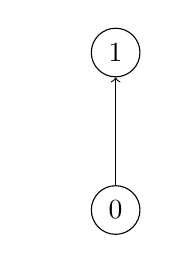
\begin{tikzpicture}
\node(pseudo) at (-1,0){};
\node(0) at (0,0)[shape=circle,draw]        {$0$};
\node(1) at (0,2)[shape=circle,draw]        {$1$};

\path [->]
  (0)      edge                 node [above]  {}     (1);

\end{tikzpicture}

Resultado: 1

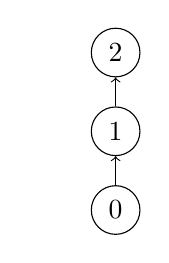
\begin{tikzpicture}
\node(pseudo) at (-1,0){};
\node(0) at (0,0)[shape=circle,draw]        {$0$};
\node(1) at (0,1)[shape=circle,draw]        {$1$};
\node(2) at (0,2)[shape=circle,draw]        {$2$};

\path [->]
  (0)      edge                 node [above]  {}     (1)
  (1)      edge                 node [above]  {}     (2);

\end{tikzpicture}

Resultado: 2

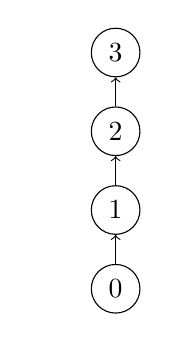
\begin{tikzpicture}
\node(pseudo) at (-1,0){};
\node(0) at (0,0)[shape=circle,draw]        {$0$};
\node(1) at (0,1)[shape=circle,draw]        {$1$};
\node(2) at (0,2)[shape=circle,draw]        {$2$};
\node(3) at (0,3)[shape=circle,draw]        {$3$};

\path [->]
  (0)      edge                 node [above]  {}     (1)
  (1)      edge                 node [above]  {}     (2)
  (2)      edge                 node [above]  {}     (3);

\end{tikzpicture}

Resultado: 3

Para el siguiente experimento buscamos observar el funcionamiento cuando existen dos caminos con el mismo largo.

\begin{tikzpicture}
\node(pseudo) at (-1,0){};
\node(0) at (2,0)[shape=circle,draw]        {$0$};
\node(1) at (0,2)[shape=circle,draw]        {$1$};
\node(2) at (0,4)[shape=circle,draw]        {$3$};
\node(3) at (2,6)[shape=circle,draw]        {$5$};
\node(4) at (4,3)[shape=circle,draw]        {$2$};
\node(5) at (4,5)[shape=circle,draw]        {$4$};

\path [->]
  (0)      edge                 node [above]  {}     (1)
  (1)      edge                 node [above]  {}     (2)
  (2)      edge                 node [above]  {}     (3)
  (0)      edge                 node [above]  {}     (4)
  (4)      edge                 node [above]  {}     (5)
  (5)      edge                 node [above]  {}     (3);
  

\end{tikzpicture}

Resultado: 3

Después repetimos lo anterior pero con la diferencia que los dos caminos son distintos en longitud.

\begin{tikzpicture}
\node(pseudo) at (-1,0){};
\node(0) at (2,0)[shape=circle,draw]        {$0$};
\node(1) at (0,1)[shape=circle,draw]        {$1$};
\node(2) at (0,2)[shape=circle,draw]        {$2$};
\node(3) at (2,9)[shape=circle,draw]        {$8$};
\node(4) at (4,3)[shape=circle,draw]        {$3$};
\node(5) at (4,5)[shape=circle,draw]        {$4$};
\node(6) at (4,6)[shape=circle,draw]        {$5$};
\node(7) at (4,7)[shape=circle,draw]        {$6$};
\node(8) at (4,8)[shape=circle,draw]        {$7$};

\path [->]
  (0)      edge                 node [above]  {}     (1)
  (1)      edge                 node [above]  {}     (2)
  (2)      edge                 node [above]  {}     (3)
  (0)      edge                 node [above]  {}     (4)
  (4)      edge                 node [above]  {}     (5)
  (5)      edge                 node [above]  {}     (6)
  (6)      edge                 node [above]  {}     (7)
  (7)      edge                 node [above]  {}     (8)
  (8)      edge                 node [above]  {}     (3);

\end{tikzpicture}

Resultado: 6 (Recorrerá el camino $0\rightarrow3\rightarrow4\rightarrow5\rightarrow6\rightarrow7\rightarrow8$ que es el más largo).

Para los siguientes experimentos lo que haremos es tener por un lado un camino corto que nos lleva del origen al destino y otro camino que nos lleve a este, pero sin comenzar
por el origen.

\begin{tikzpicture}
\node(pseudo) at (-1,0){};
\node(0) at (2,0)[shape=circle,draw]        {$0$};
\node(1) at (4,1)[shape=circle,draw]        {$1$};
\node(2) at (4,2)[shape=circle,draw]        {$2$};
\node(3) at (4,3)[shape=circle,draw]        {$3$};
\node(4) at (0,4)[shape=circle,draw]        {$4$};
\node(5) at (2,5)[shape=circle,draw]        {$5$};


\path [->]
  (0)      edge                 node [above]  {}     (4)
  (1)      edge                 node [above]  {}     (2)
  (2)      edge                 node [above]  {}     (3)
  (3)      edge                 node [above]  {}     (5)
  (4)      edge                 node [above]  {}     (5);


\end{tikzpicture}

Resultado: 2.

\begin{tikzpicture}
\node(pseudo) at (-1,0){};
\node(0) at (2,0)[shape=circle,draw]        {$0$};
\node(1) at (4,1)[shape=circle,draw]        {$1$};
\node(2) at (4,2)[shape=circle,draw]        {$2$};
\node(3) at (4,3)[shape=circle,draw]        {$3$};
\node(4) at (4,4)[shape=circle,draw]        {$4$};
\node(5) at (2,5)[shape=circle,draw]        {$5$};


\path [->]
  (0)      edge                 node [above]  {}     (5)
  (1)      edge                 node [above]  {}     (2)
  (2)      edge                 node [above]  {}     (3)
  (3)      edge                 node [above]  {}     (4);

\end{tikzpicture}

Resultado: 1.

Como podemos ver la idea es que tenga por resultado la cantidad de portales que tiene que atravesar en el camino que comienza en el origen y concluye en el destino, y no
los que no cumplan esta última propiedad.

Lo siguiente serán unos tests dedicados a la medición de tiempos. Graficaremos los casos por separado y con distintos tamaños ya que la diferencia de tiempos entre el mejor y peor caso es demasiado
grande como para ponerlos en un solo gráfico, ya que se perderían detalles.

En estas mediciones no consideramos el tiempo de incialización, que consideramos parte de la lectura de la entrada.

 Comenzemos por el peor caso el cual conseguimos mediante un grafo completo, por completo nos 
refirimos a que cada piso tiene un portal por cada uno de los siguientes. Con más posibilidades debemos que tener en cuenta todas para obtener el camino con mayor número 
de portales. Para el caso promedio simplemente nos armaremos un grafo aleatorio que partirá de la base que del caso anterior, osea que hay un camino que involucra a todos los 
nodos y agregaremos aristas entre los nodos de forma aleatoria. El tamaño de las muestra variara entre 200 y 290 con saltos de 10.

\begin{figure}[H]
\input{plots/Tp2Ej1ExpPeor.tex}
\caption{Comparación de tiempos variando la cantidad de pisos}
\end{figure}

Para el mejor caso, podríamos simplemente un grafo similar al del último test de correctitud. En otras palabras que el comienzo este unido con el fin y los nodos intermedios 
no influyan. Dado que este caso es poco interesante porque solamente hay una posibilidad y el tiempo sería constante, hemos decidido omitir este caso como trivial y asumir que el 
mejor caso a evaluar es en el cual exista un camino entre el primero y el último que pase por todos los nodos(semejante a los primeros tests de correctitud). Variaremos el 
tamaño de las muestras de 200 a 2000 con saltos de 200. Usamos esta muestra tan grande porque usando la anterior no nos permite apreciar suficiente diferencia.

\begin{figure}[H]
\input{plots/Tp2Ej1ExpMejor.tex}
\caption{Comparación de tiempos variando la cantidad de pisos}
\end{figure}


